%! Author = evandro
%! Date = 13/02/21

% Preamble
\providecommand{\report}{..}
\documentclass[../main.tex]{subfiles}

% Packages

% Document
\begin{document}
    \chapter{Descrizione del modello}\label{ch:descrizione-del-modello}
    Il modello sviluppato è stato implementato usando l'applicativo \textit{JSIMgraph}.

    \section{Formalizzazione del problema}\label{sec:formalizzazione-del-problema}
    Partendo dalla descrizione del problema, si è deciso di sviluppare un modello multi-classe con tre stazioni di coda.
    Ogni stazione di coda rappresenta un diverso componente dell'architettura \textit{three tier}.
    Le stazioni di coda sono disposte in sequenza: stazione del \textit{web server}, la stazione del
    \textit{application server} e infine la stazione del \textit{database}.
    \newline
    In particolare, ogni stazione è caratterizzata da una coda limitata e dal numero di repliche.
    Al termine della sequenza delle tre stazioni di coda, i diversi \textit{jobs} vengono instradati verso il
    \textit{web server}.

    \begin{figure}[H]
        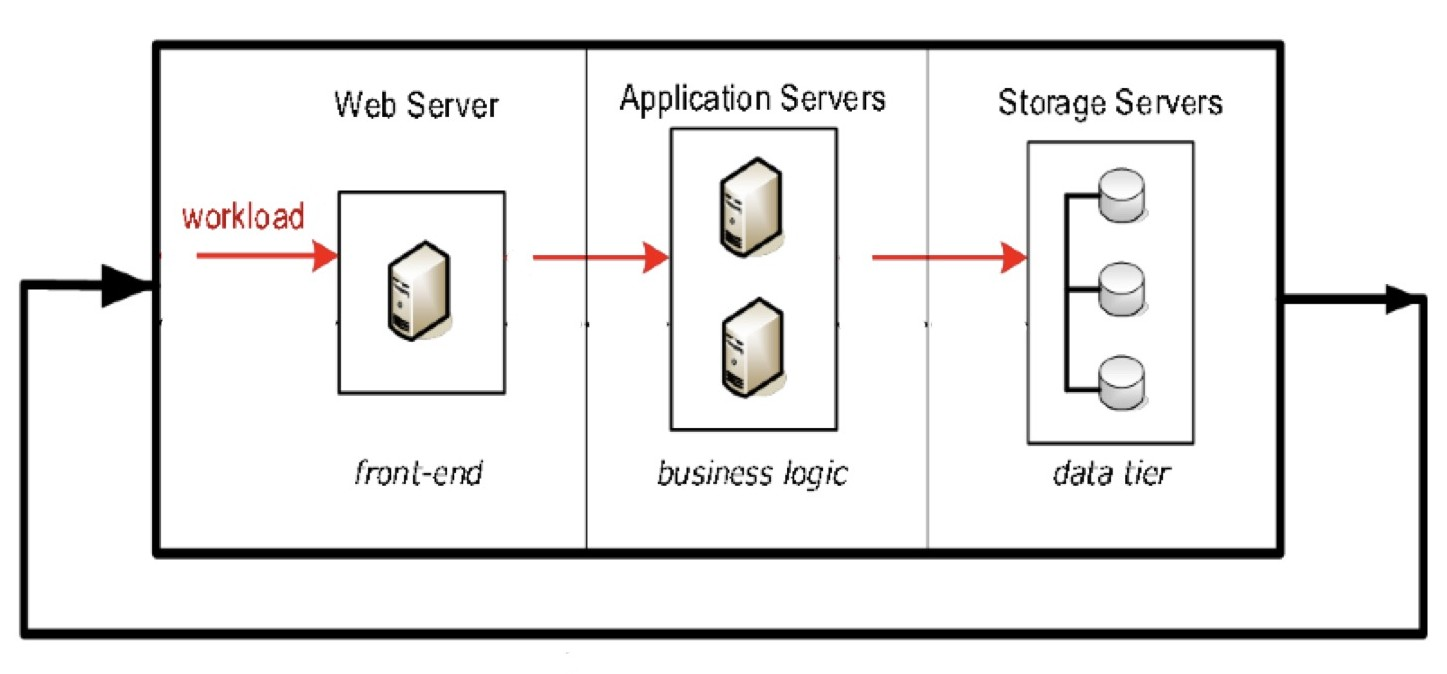
\includegraphics[scale = 0.3]{assets/three_tier}\\
        \caption[\textit{Architettura} alto livello]{architetture del modello di alto livello.}
        \label{fig:architettura-alto-livello-modello}
    \end{figure}


    \section{Le classi}\label{sec:le-classi}
    I \textit{jobs} che circolano nel sistema sonno stati identificati con tre diverse classi: tutti i \textit{jobs}
    che appartengono alla stessa classe, sono caratterizzati dalle stesse proprietà.
    \begin{itemize}
        \item \textbf{N\textsubscript{U}} richieste dell'utente (caratterizzate da un \textit{think time} Z\textsubscript{U}).
        \item \textbf{N\textsubscript{S}} requisiti software di chiamata di procedura remota;
        \item \textbf{N\textsubscript{B}} programmi di collaborazione.
    \end{itemize}
    Tutte e tre le classi sono di tipo chiuso e sono caratterizzate da una diversa popolazione (numero di \textit{jobs}).
    Tuttavia solo la classe richieste dell'utente (U), presenta un \textit{think time}. Questa specifica è gestita
    tramite una stazione di ritardo.
    La \textit{reference station} per la classe chiamata di procedura remota (S) e per la classe programmi di collaborazione
    (B), è la stazione \textit{web server}; metre per la classe (richieste dell'utente) è la stazione di ritardo.
    \begin{figure}[H]
        \centering
        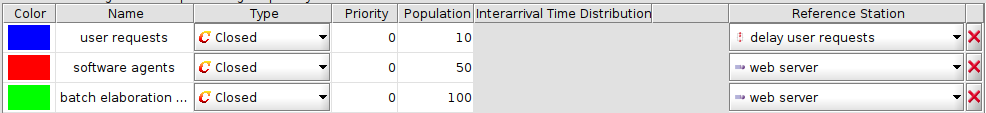
\includegraphics[scale = 0.5]{assets/classes.png}\\
        \caption[\textit{Classi} del sistema]{classi presenti nel sistema.}
        \label{fig:clssi-del-sistema}
    \end{figure}


    \section{L'architettura del modello completo}\label{sec:l'architettura-del-modello-completo}
    Nel modello sono presenti le tre stazioni coda, ciascuna per ogni componente del sistema, disposte in cascate;
    a valle troviamo il \textit{router} collegato sia alla stazione di ritardo e sia al \textit{web server}.

    \begin{figure}[H]
        \centering
        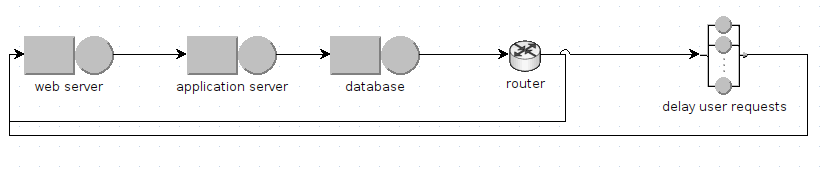
\includegraphics[scale = 0.6]{assets/modello_jsim}\\
        \caption[\textit{Architettura} del modello]{architettura del modello completo.}
        \label{fig:architettura-del-modello-completo}
    \end{figure}

    \subsection{Le componenti del modello}\label{subsec:le-componenti-del-modello}
    A livello architettonico si possono distinguere quattro stazioni ed un router.
    Tutte le stazioni di coda hanno una capacità limitata e questo implica l'adozione di una politica di gestione nel
    caso la capacità massima venga ragiunta.
    La regola utilizzata è \textit{blocking after service (BAS)} per rispettare al meglio le richieste del problema.
    La politica di selezione del prossimo \textit{job} (o di coda) adottata è una  \textit{non-preemptive} di tipo \textit{first come first served (FCFS)}.
    \begin{figure}[H]
        \centering
        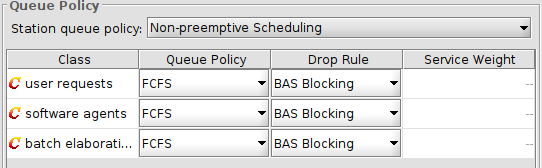
\includegraphics[scale = 0.5]{assets/queue_policy.png}\\
        \caption[\textit{Politica} di gestione delle code]{ politica di gestione delle code adottata nelle stazioni di coda (\textit{web server}, \textit{application server}, \textit{database})}
        \label{fig:politica-di-coda}
    \end{figure}
    La distribuzione del \textit{service time} segue una esponenziale la cui media è pari ai valori riportati in tabella [\ref{tab:tempo-richiesto-da-ogni-risorsa-per-tipo-di-richiesta}].
    Analizzando il modello da sinistra verso destra, rispettando l'ordine di visita delle stazioni, si identificano:
    \begin{itemize}
        \item stazione di coda, \textit{"web server"}.
        \item stazione di coda, \textit{"application server"}.
        \item stazione di coda, \textit{"database"}.
        \item router, \textit{"router"}. Utilizza una stategia probabilistica per indirizzare i diversi \textit{jobs} presenti nel sistema in base alla loro classe di appartenenza.
        Se un \textit{job} appartiene alla classe chiamata di procedura remota (S) oppure alla classe programmi di collaborazione (B), essi sono indirizzati al \textit{web server} con probabilità uno;
        se invece il \textit{job} è dela classe richieste dell' utente (U), esso è indirizzato con probabilità uno alla stazione di ritardo. \footnote{il router puo anche essere eliminato in quanto le sue funzionalità possono essere svolte dalla politica di \textit{routing} del \textit{database}. Tuttavia la sua presenza è giustificata da una maggiore leggibilità del modello.}
        \item stazione di ritardo, \textit{"delay user request"}. La distribuzione del \textit{service time} segue una esponenziale la cui media è pari a \textit{12000 ms};
        essa equivale al \textit{think time} della classe richieste dell'utente (U).

    \end{itemize}



\end{document}